\section{Modelo de Processo}

Nesta seção é proposto um modelo para a gerência de ordens de serviço. Tal
modelo busca ser aderente às recomendações da IN4 mas busca ao mesmo tempo
possibilitar a customização para as necessidades específicas do órgão que vier
a adotá-lo.

A figura \ref{fig:so_process} mostra o desenho do processo proposto, sua
sequência e as etapas envolvidas.

\begin{figure}[h]
  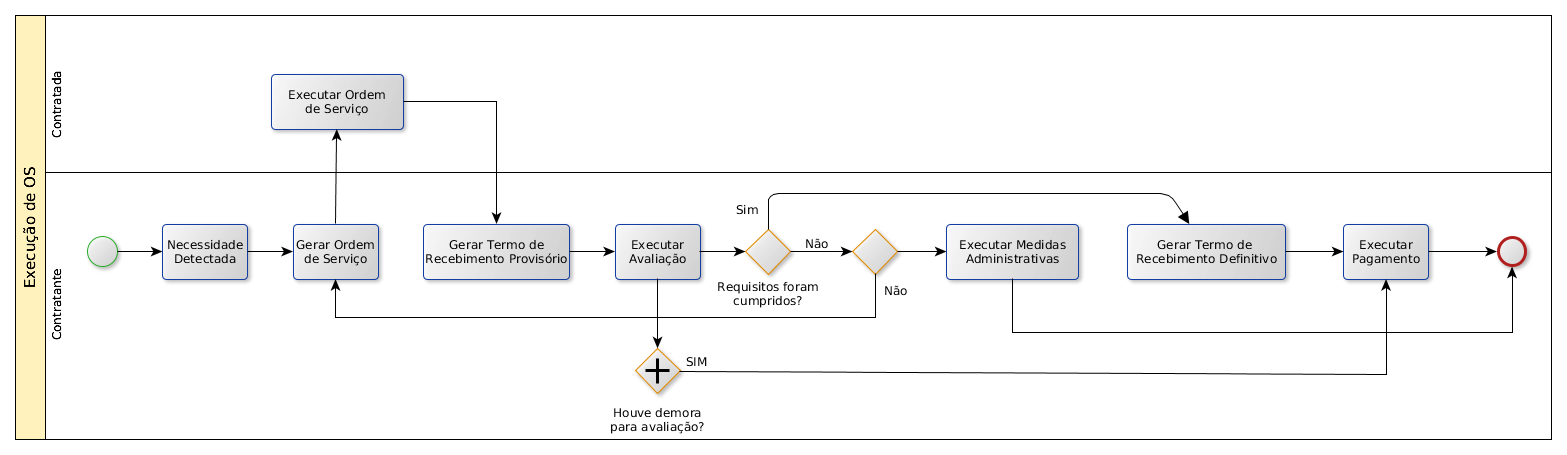
\includegraphics[width=1.0\textwidth,natwidth=500,natheight=150]{figures/so_process.png}
  \caption{Proposta de um processo para gerenciar ordens de serviço.}
  \label{fig:so_process}
\end{figure}

As atividades do processo são descritas a seguir:

\begin{itemize}
  \item \textbf{Necessidade Detectada:} uma necessidade foi encontrada e o
  sistema atual não é capaz de supri-la. Nesse caso deve-se formalmente criar
  um pedido para alteração e/ou aquisição de um \textit{software};
  \item \textbf{Gerar Ordem de Serviço:} com base na descrição da necessidade é
  criada, então, a ordem de serviço. A OS deve contemplar a necessidade, os
  critérios de avaliação, envolvidos, custos e prazos;
  \item \textbf{Executar Ordem de Serviço:} uma vez quea ordem de serviço tenha
  sido criada e aprovada ela será então encaminhada à prestadora de serviços. É
  de responsabilidade da prestadora toda a execução no que diz respeito à
  organização interna, tecnologias envolvidas e metodologias empregadas.
  \item \textbf{Gerar Termo de Recebimento Provisório:} quando a prestadora
  finaliza o desenvolvimento da ordem de serviço ela deve informar a contratante,
  que deverá, então, gerar o Termo de Recebimento Provisório. Tal termo atesta
  que a prestadora executou o serviço e que partir daquele momento ela aguarda
  a avaliação dos itens desenvolvidos.
  \item \textbf{Executar Avaliação:} ao gerar o Termo de Recebimento Provisório,
  a contratante tem a responsabilidade de avaliar o produto desenvolvido, isto é,
  verificar se tudo o que foi desenvolvido está de acordo com o que foi previsto
  na OS.
  \item \textbf{Tomar Medidas Administrativas:} no caso em que a prestadora
  continuamente não cumpre com os objetivos previstos na OS, o que inclui
  indicadores de qualidae, a contratante poderá tomar medidas adminstrativas,
  como a aplicação e multas ou até mesmo o cancelameto da OS.
  \item \textbf{Gerar Termo de Recebimento Definitivo:} se a OS foi corretamente
  executada e os itens entregues correspondem às expectativas descritas na
  OS a contratante deverá então gerar o Termo de Recebimento Definitivo, que
  atesta que a prestadora executou a ordem de serviço e que todos os itens
  acordados na OS foram entregues.
  \item \textbf{Executar Pagamento:} por fim, uma vez que o Termo de Recebimento
  definitivo foi emitido é então possível executar o pagamento à prestadora.
\end{itemize}
